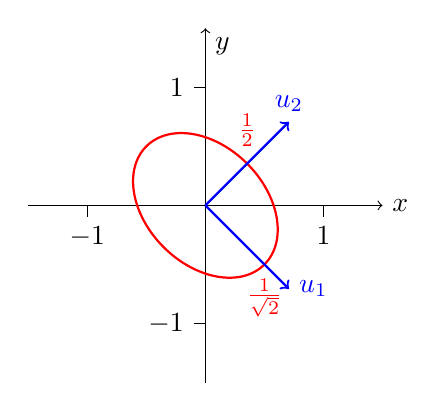
\begin{tikzpicture}[scale=1.5]
        \begin{scope}[color=black]
          \draw[->] (-1.5,0) -- (1.5,0) node[right] {$x$};
          \draw[->] (0,-1.5) -- (0,1.5) node[below right] {$y$};
          \draw (-1,0) -- +(0,-.1) node[below] {$-1$};
          \draw (1,0) -- +(0,-.1) node[below] {$1$};
          \draw (0,-1) -- +(-.1,0) node[left] {$-1$};
          \draw (0,1) -- +(-.1,0) node[left] {$1$};
        \end{scope}
        \begin{scope}[color=blue,cm={(1/sqrt(2),-1/sqrt(2),1/sqrt(2),1/sqrt(2),(0,0))}]
          \draw[thick,red] (0,0) circle [x radius={1/sqrt(2)}, y radius={1/2}];
          \draw[red] ({1/sqrt(2)},0) +(0.2,-0.2) node {$\frac{1}{\sqrt{2}}$};
          \draw[red] (0,{1/2}) +(-0.2,0.2) node {$\frac{1}{2}$};
          \draw[thick,blue,->] (0,0) -- (1,0) node[right] {$\vect{u}_1$};
          \draw[thick,blue,->] (0,0) -- (0,1) node[above] {$\vect{u}_2$};
        \end{scope}
      \end{tikzpicture}
